% Graphic for TeX using PGF
% Title: /home/budnyjj/univer/GIT/discipline/SPO/lab_6/report/img/dependencies.dia
% Creator: Dia v0.97.2
% CreationDate: Wed May 14 17:56:28 2014
% For: budnyjj
% \usepackage{tikz}
% The following commands are not supported in PSTricks at present
% We define them conditionally, so when they are implemented,
% this pgf file will use them.
\ifx\du\undefined
  \newlength{\du}
\fi
\setlength{\du}{15\unitlength}
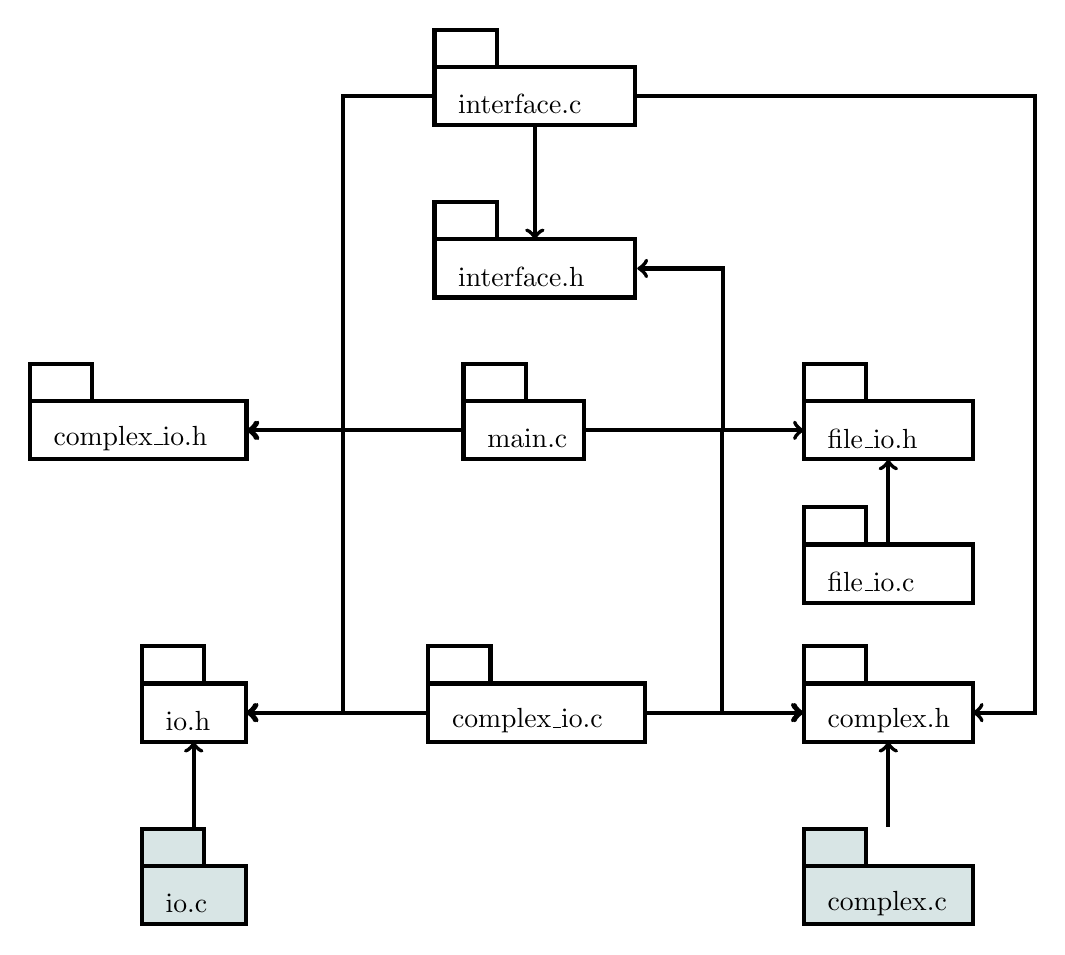
\begin{tikzpicture}
\pgftransformxscale{1.000000}
\pgftransformyscale{-1.000000}
\definecolor{dialinecolor}{rgb}{0.000000, 0.000000, 0.000000}
\pgfsetstrokecolor{dialinecolor}
\definecolor{dialinecolor}{rgb}{1.000000, 1.000000, 1.000000}
\pgfsetfillcolor{dialinecolor}
\pgfsetlinewidth{0.100000\du}
\pgfsetdash{}{0pt}
\definecolor{dialinecolor}{rgb}{1.000000, 1.000000, 1.000000}
\pgfsetfillcolor{dialinecolor}
\fill (36.000000\du,33.400000\du)--(36.000000\du,34.800000\du)--(40.065000\du,34.800000\du)--(40.065000\du,33.400000\du)--cycle;
\definecolor{dialinecolor}{rgb}{0.000000, 0.000000, 0.000000}
\pgfsetstrokecolor{dialinecolor}
\draw (36.000000\du,33.400000\du)--(36.000000\du,34.800000\du)--(40.065000\du,34.800000\du)--(40.065000\du,33.400000\du)--cycle;
\definecolor{dialinecolor}{rgb}{1.000000, 1.000000, 1.000000}
\pgfsetfillcolor{dialinecolor}
\fill (36.000000\du,32.500000\du)--(36.000000\du,33.400000\du)--(37.500000\du,33.400000\du)--(37.500000\du,32.500000\du)--cycle;
\definecolor{dialinecolor}{rgb}{0.000000, 0.000000, 0.000000}
\pgfsetstrokecolor{dialinecolor}
\draw (36.000000\du,32.500000\du)--(36.000000\du,33.400000\du)--(37.500000\du,33.400000\du)--(37.500000\du,32.500000\du)--cycle;
% setfont left to latex
\definecolor{dialinecolor}{rgb}{0.000000, 0.000000, 0.000000}
\pgfsetstrokecolor{dialinecolor}
\node[anchor=west] at (36.300000\du,34.295000\du){complex.h};
\pgfsetlinewidth{0.100000\du}
\pgfsetdash{}{0pt}
\definecolor{dialinecolor}{rgb}{1.000000, 1.000000, 1.000000}
\pgfsetfillcolor{dialinecolor}
\fill (17.350000\du,26.600000\du)--(17.350000\du,28.000000\du)--(22.570000\du,28.000000\du)--(22.570000\du,26.600000\du)--cycle;
\definecolor{dialinecolor}{rgb}{0.000000, 0.000000, 0.000000}
\pgfsetstrokecolor{dialinecolor}
\draw (17.350000\du,26.600000\du)--(17.350000\du,28.000000\du)--(22.570000\du,28.000000\du)--(22.570000\du,26.600000\du)--cycle;
\definecolor{dialinecolor}{rgb}{1.000000, 1.000000, 1.000000}
\pgfsetfillcolor{dialinecolor}
\fill (17.350000\du,25.700000\du)--(17.350000\du,26.600000\du)--(18.850000\du,26.600000\du)--(18.850000\du,25.700000\du)--cycle;
\definecolor{dialinecolor}{rgb}{0.000000, 0.000000, 0.000000}
\pgfsetstrokecolor{dialinecolor}
\draw (17.350000\du,25.700000\du)--(17.350000\du,26.600000\du)--(18.850000\du,26.600000\du)--(18.850000\du,25.700000\du)--cycle;
% setfont left to latex
\definecolor{dialinecolor}{rgb}{0.000000, 0.000000, 0.000000}
\pgfsetstrokecolor{dialinecolor}
\node[anchor=west] at (17.650000\du,27.495000\du){complex\_io.h};
\pgfsetlinewidth{0.100000\du}
\pgfsetdash{}{0pt}
\definecolor{dialinecolor}{rgb}{1.000000, 1.000000, 1.000000}
\pgfsetfillcolor{dialinecolor}
\fill (36.000000\du,26.600000\du)--(36.000000\du,28.000000\du)--(40.065000\du,28.000000\du)--(40.065000\du,26.600000\du)--cycle;
\definecolor{dialinecolor}{rgb}{0.000000, 0.000000, 0.000000}
\pgfsetstrokecolor{dialinecolor}
\draw (36.000000\du,26.600000\du)--(36.000000\du,28.000000\du)--(40.065000\du,28.000000\du)--(40.065000\du,26.600000\du)--cycle;
\definecolor{dialinecolor}{rgb}{1.000000, 1.000000, 1.000000}
\pgfsetfillcolor{dialinecolor}
\fill (36.000000\du,25.700000\du)--(36.000000\du,26.600000\du)--(37.500000\du,26.600000\du)--(37.500000\du,25.700000\du)--cycle;
\definecolor{dialinecolor}{rgb}{0.000000, 0.000000, 0.000000}
\pgfsetstrokecolor{dialinecolor}
\draw (36.000000\du,25.700000\du)--(36.000000\du,26.600000\du)--(37.500000\du,26.600000\du)--(37.500000\du,25.700000\du)--cycle;
% setfont left to latex
\definecolor{dialinecolor}{rgb}{0.000000, 0.000000, 0.000000}
\pgfsetstrokecolor{dialinecolor}
\node[anchor=west] at (36.300000\du,27.495000\du){file\_io.h};
\pgfsetlinewidth{0.100000\du}
\pgfsetdash{}{0pt}
\definecolor{dialinecolor}{rgb}{1.000000, 1.000000, 1.000000}
\pgfsetfillcolor{dialinecolor}
\fill (27.100000\du,22.700000\du)--(27.100000\du,24.100000\du)--(31.935000\du,24.100000\du)--(31.935000\du,22.700000\du)--cycle;
\definecolor{dialinecolor}{rgb}{0.000000, 0.000000, 0.000000}
\pgfsetstrokecolor{dialinecolor}
\draw (27.100000\du,22.700000\du)--(27.100000\du,24.100000\du)--(31.935000\du,24.100000\du)--(31.935000\du,22.700000\du)--cycle;
\definecolor{dialinecolor}{rgb}{1.000000, 1.000000, 1.000000}
\pgfsetfillcolor{dialinecolor}
\fill (27.100000\du,21.800000\du)--(27.100000\du,22.700000\du)--(28.600000\du,22.700000\du)--(28.600000\du,21.800000\du)--cycle;
\definecolor{dialinecolor}{rgb}{0.000000, 0.000000, 0.000000}
\pgfsetstrokecolor{dialinecolor}
\draw (27.100000\du,21.800000\du)--(27.100000\du,22.700000\du)--(28.600000\du,22.700000\du)--(28.600000\du,21.800000\du)--cycle;
% setfont left to latex
\definecolor{dialinecolor}{rgb}{0.000000, 0.000000, 0.000000}
\pgfsetstrokecolor{dialinecolor}
\node[anchor=west] at (27.400000\du,23.595000\du){interface.h};
\pgfsetlinewidth{0.100000\du}
\pgfsetdash{}{0pt}
\definecolor{dialinecolor}{rgb}{1.000000, 1.000000, 1.000000}
\pgfsetfillcolor{dialinecolor}
\fill (20.050000\du,33.400000\du)--(20.050000\du,34.800000\du)--(22.550000\du,34.800000\du)--(22.550000\du,33.400000\du)--cycle;
\definecolor{dialinecolor}{rgb}{0.000000, 0.000000, 0.000000}
\pgfsetstrokecolor{dialinecolor}
\draw (20.050000\du,33.400000\du)--(20.050000\du,34.800000\du)--(22.550000\du,34.800000\du)--(22.550000\du,33.400000\du)--cycle;
\definecolor{dialinecolor}{rgb}{1.000000, 1.000000, 1.000000}
\pgfsetfillcolor{dialinecolor}
\fill (20.050000\du,32.500000\du)--(20.050000\du,33.400000\du)--(21.550000\du,33.400000\du)--(21.550000\du,32.500000\du)--cycle;
\definecolor{dialinecolor}{rgb}{0.000000, 0.000000, 0.000000}
\pgfsetstrokecolor{dialinecolor}
\draw (20.050000\du,32.500000\du)--(20.050000\du,33.400000\du)--(21.550000\du,33.400000\du)--(21.550000\du,32.500000\du)--cycle;
% setfont left to latex
\definecolor{dialinecolor}{rgb}{0.000000, 0.000000, 0.000000}
\pgfsetstrokecolor{dialinecolor}
\node[anchor=west] at (20.350000\du,34.295000\du){io.h};
\pgfsetlinewidth{0.100000\du}
\pgfsetdash{}{0pt}
\definecolor{dialinecolor}{rgb}{1.000000, 1.000000, 1.000000}
\pgfsetfillcolor{dialinecolor}
\fill (26.950000\du,33.400000\du)--(26.950000\du,34.800000\du)--(32.170000\du,34.800000\du)--(32.170000\du,33.400000\du)--cycle;
\definecolor{dialinecolor}{rgb}{0.000000, 0.000000, 0.000000}
\pgfsetstrokecolor{dialinecolor}
\draw (26.950000\du,33.400000\du)--(26.950000\du,34.800000\du)--(32.170000\du,34.800000\du)--(32.170000\du,33.400000\du)--cycle;
\definecolor{dialinecolor}{rgb}{1.000000, 1.000000, 1.000000}
\pgfsetfillcolor{dialinecolor}
\fill (26.950000\du,32.500000\du)--(26.950000\du,33.400000\du)--(28.450000\du,33.400000\du)--(28.450000\du,32.500000\du)--cycle;
\definecolor{dialinecolor}{rgb}{0.000000, 0.000000, 0.000000}
\pgfsetstrokecolor{dialinecolor}
\draw (26.950000\du,32.500000\du)--(26.950000\du,33.400000\du)--(28.450000\du,33.400000\du)--(28.450000\du,32.500000\du)--cycle;
% setfont left to latex
\definecolor{dialinecolor}{rgb}{0.000000, 0.000000, 0.000000}
\pgfsetstrokecolor{dialinecolor}
\node[anchor=west] at (27.250000\du,34.295000\du){complex\_io.c};
\pgfsetlinewidth{0.100000\du}
\pgfsetdash{}{0pt}
\definecolor{dialinecolor}{rgb}{1.000000, 1.000000, 1.000000}
\pgfsetfillcolor{dialinecolor}
\fill (27.800000\du,26.600000\du)--(27.800000\du,28.000000\du)--(30.710000\du,28.000000\du)--(30.710000\du,26.600000\du)--cycle;
\definecolor{dialinecolor}{rgb}{0.000000, 0.000000, 0.000000}
\pgfsetstrokecolor{dialinecolor}
\draw (27.800000\du,26.600000\du)--(27.800000\du,28.000000\du)--(30.710000\du,28.000000\du)--(30.710000\du,26.600000\du)--cycle;
\definecolor{dialinecolor}{rgb}{1.000000, 1.000000, 1.000000}
\pgfsetfillcolor{dialinecolor}
\fill (27.800000\du,25.700000\du)--(27.800000\du,26.600000\du)--(29.300000\du,26.600000\du)--(29.300000\du,25.700000\du)--cycle;
\definecolor{dialinecolor}{rgb}{0.000000, 0.000000, 0.000000}
\pgfsetstrokecolor{dialinecolor}
\draw (27.800000\du,25.700000\du)--(27.800000\du,26.600000\du)--(29.300000\du,26.600000\du)--(29.300000\du,25.700000\du)--cycle;
% setfont left to latex
\definecolor{dialinecolor}{rgb}{0.000000, 0.000000, 0.000000}
\pgfsetstrokecolor{dialinecolor}
\node[anchor=west] at (28.100000\du,27.495000\du){main.c};
\pgfsetlinewidth{0.100000\du}
\pgfsetbuttcap
\pgfsetdash{}{0pt}
{
\definecolor{dialinecolor}{rgb}{0.000000, 0.000000, 0.000000}
\pgfsetfillcolor{dialinecolor}
% was here!!!
\pgfsetarrowsend{to}
\definecolor{dialinecolor}{rgb}{0.000000, 0.000000, 0.000000}
\pgfsetstrokecolor{dialinecolor}
\draw (27.753716\du,27.300000\du)--(24.900000\du,27.300000\du)--(24.900000\du,34.100000\du)--(22.550000\du,34.100000\du);
}
% setfont left to latex
\pgfsetlinewidth{0.100000\du}
\pgfsetbuttcap
\pgfsetdash{}{0pt}
{
\definecolor{dialinecolor}{rgb}{0.000000, 0.000000, 0.000000}
\pgfsetfillcolor{dialinecolor}
% was here!!!
\pgfsetarrowsend{to}
\definecolor{dialinecolor}{rgb}{0.000000, 0.000000, 0.000000}
\pgfsetstrokecolor{dialinecolor}
\draw (30.759491\du,27.300000\du)--(34.030200\du,27.300000\du)--(34.030200\du,34.100000\du)--(36.000000\du,34.100000\du);
}
% setfont left to latex
\pgfsetlinewidth{0.100000\du}
\pgfsetbuttcap
\pgfsetdash{}{0pt}
{
\definecolor{dialinecolor}{rgb}{0.000000, 0.000000, 0.000000}
\pgfsetfillcolor{dialinecolor}
% was here!!!
\pgfsetarrowsend{to}
\definecolor{dialinecolor}{rgb}{0.000000, 0.000000, 0.000000}
\pgfsetstrokecolor{dialinecolor}
\draw (30.760367\du,27.300000\du)--(31.260367\du,27.300000\du)--(35.500000\du,27.300000\du)--(36.000000\du,27.300000\du);
}
% setfont left to latex
\pgfsetlinewidth{0.100000\du}
\pgfsetbuttcap
\pgfsetdash{}{0pt}
{
\definecolor{dialinecolor}{rgb}{0.000000, 0.000000, 0.000000}
\pgfsetfillcolor{dialinecolor}
% was here!!!
\pgfsetarrowsend{to}
\definecolor{dialinecolor}{rgb}{0.000000, 0.000000, 0.000000}
\pgfsetstrokecolor{dialinecolor}
\draw (27.800000\du,27.300000\du)--(27.300000\du,27.300000\du)--(23.070000\du,27.300000\du)--(22.570000\du,27.300000\du);
}
% setfont left to latex
\pgfsetlinewidth{0.100000\du}
\pgfsetbuttcap
\pgfsetdash{}{0pt}
{
\definecolor{dialinecolor}{rgb}{0.000000, 0.000000, 0.000000}
\pgfsetfillcolor{dialinecolor}
% was here!!!
\pgfsetarrowsend{to}
\definecolor{dialinecolor}{rgb}{0.000000, 0.000000, 0.000000}
\pgfsetstrokecolor{dialinecolor}
\draw (30.759291\du,27.300000\du)--(34.050000\du,27.300000\du)--(34.050000\du,23.400000\du)--(31.984039\du,23.400000\du);
}
% setfont left to latex
\pgfsetlinewidth{0.100000\du}
\pgfsetbuttcap
\pgfsetdash{}{0pt}
{
\definecolor{dialinecolor}{rgb}{0.000000, 0.000000, 0.000000}
\pgfsetfillcolor{dialinecolor}
% was here!!!
\pgfsetarrowsend{to}
\definecolor{dialinecolor}{rgb}{0.000000, 0.000000, 0.000000}
\pgfsetstrokecolor{dialinecolor}
\draw (26.899675\du,34.100000\du)--(26.399675\du,34.100000\du)--(23.100317\du,34.100000\du)--(22.600317\du,34.100000\du);
}
% setfont left to latex
\pgfsetlinewidth{0.100000\du}
\pgfsetbuttcap
\pgfsetdash{}{0pt}
{
\definecolor{dialinecolor}{rgb}{0.000000, 0.000000, 0.000000}
\pgfsetfillcolor{dialinecolor}
% was here!!!
\pgfsetarrowsend{to}
\definecolor{dialinecolor}{rgb}{0.000000, 0.000000, 0.000000}
\pgfsetstrokecolor{dialinecolor}
\draw (32.220325\du,34.100000\du)--(32.720325\du,34.100000\du)--(35.449746\du,34.100000\du)--(35.949746\du,34.100000\du);
}
% setfont left to latex
\pgfsetlinewidth{0.100000\du}
\pgfsetdash{}{0pt}
\definecolor{dialinecolor}{rgb}{1.000000, 1.000000, 1.000000}
\pgfsetfillcolor{dialinecolor}
\fill (27.100000\du,18.550000\du)--(27.100000\du,19.950000\du)--(31.935000\du,19.950000\du)--(31.935000\du,18.550000\du)--cycle;
\definecolor{dialinecolor}{rgb}{0.000000, 0.000000, 0.000000}
\pgfsetstrokecolor{dialinecolor}
\draw (27.100000\du,18.550000\du)--(27.100000\du,19.950000\du)--(31.935000\du,19.950000\du)--(31.935000\du,18.550000\du)--cycle;
\definecolor{dialinecolor}{rgb}{1.000000, 1.000000, 1.000000}
\pgfsetfillcolor{dialinecolor}
\fill (27.100000\du,17.650000\du)--(27.100000\du,18.550000\du)--(28.600000\du,18.550000\du)--(28.600000\du,17.650000\du)--cycle;
\definecolor{dialinecolor}{rgb}{0.000000, 0.000000, 0.000000}
\pgfsetstrokecolor{dialinecolor}
\draw (27.100000\du,17.650000\du)--(27.100000\du,18.550000\du)--(28.600000\du,18.550000\du)--(28.600000\du,17.650000\du)--cycle;
% setfont left to latex
\definecolor{dialinecolor}{rgb}{0.000000, 0.000000, 0.000000}
\pgfsetstrokecolor{dialinecolor}
\node[anchor=west] at (27.400000\du,19.445000\du){interface.c};
\pgfsetlinewidth{0.100000\du}
\pgfsetbuttcap
\pgfsetdash{}{0pt}
{
\definecolor{dialinecolor}{rgb}{0.000000, 0.000000, 0.000000}
\pgfsetfillcolor{dialinecolor}
% was here!!!
\pgfsetarrowsend{to}
\definecolor{dialinecolor}{rgb}{0.000000, 0.000000, 0.000000}
\pgfsetstrokecolor{dialinecolor}
\draw (29.517500\du,20.000366\du)--(29.517500\du,20.500366\du)--(29.517500\du,22.200000\du)--(29.517500\du,22.700000\du);
}
% setfont left to latex
\pgfsetlinewidth{0.100000\du}
\pgfsetbuttcap
\pgfsetdash{}{0pt}
{
\definecolor{dialinecolor}{rgb}{0.000000, 0.000000, 0.000000}
\pgfsetfillcolor{dialinecolor}
% was here!!!
\pgfsetarrowsend{to}
\definecolor{dialinecolor}{rgb}{0.000000, 0.000000, 0.000000}
\pgfsetstrokecolor{dialinecolor}
\draw (27.050362\du,19.250000\du)--(24.900000\du,19.250000\du)--(24.900000\du,27.300000\du)--(22.619351\du,27.300000\du);
}
% setfont left to latex
\pgfsetlinewidth{0.100000\du}
\pgfsetbuttcap
\pgfsetdash{}{0pt}
{
\definecolor{dialinecolor}{rgb}{0.000000, 0.000000, 0.000000}
\pgfsetfillcolor{dialinecolor}
% was here!!!
\pgfsetarrowsend{to}
\definecolor{dialinecolor}{rgb}{0.000000, 0.000000, 0.000000}
\pgfsetstrokecolor{dialinecolor}
\draw (31.985301\du,19.250000\du)--(41.565000\du,19.250000\du)--(41.565000\du,34.100000\du)--(40.065000\du,34.100000\du);
}
% setfont left to latex
\pgfsetlinewidth{0.100000\du}
\pgfsetdash{}{0pt}
\definecolor{dialinecolor}{rgb}{0.847059, 0.898039, 0.898039}
\pgfsetfillcolor{dialinecolor}
\fill (36.000000\du,37.800000\du)--(36.000000\du,39.200000\du)--(40.065000\du,39.200000\du)--(40.065000\du,37.800000\du)--cycle;
\definecolor{dialinecolor}{rgb}{0.000000, 0.000000, 0.000000}
\pgfsetstrokecolor{dialinecolor}
\draw (36.000000\du,37.800000\du)--(36.000000\du,39.200000\du)--(40.065000\du,39.200000\du)--(40.065000\du,37.800000\du)--cycle;
\definecolor{dialinecolor}{rgb}{0.847059, 0.898039, 0.898039}
\pgfsetfillcolor{dialinecolor}
\fill (36.000000\du,36.900000\du)--(36.000000\du,37.800000\du)--(37.500000\du,37.800000\du)--(37.500000\du,36.900000\du)--cycle;
\definecolor{dialinecolor}{rgb}{0.000000, 0.000000, 0.000000}
\pgfsetstrokecolor{dialinecolor}
\draw (36.000000\du,36.900000\du)--(36.000000\du,37.800000\du)--(37.500000\du,37.800000\du)--(37.500000\du,36.900000\du)--cycle;
% setfont left to latex
\definecolor{dialinecolor}{rgb}{0.000000, 0.000000, 0.000000}
\pgfsetstrokecolor{dialinecolor}
\node[anchor=west] at (36.300000\du,38.695000\du){complex.c};
\pgfsetlinewidth{0.100000\du}
\pgfsetdash{}{0pt}
\definecolor{dialinecolor}{rgb}{0.847059, 0.898039, 0.898039}
\pgfsetfillcolor{dialinecolor}
\fill (20.050000\du,37.800000\du)--(20.050000\du,39.200000\du)--(22.550000\du,39.200000\du)--(22.550000\du,37.800000\du)--cycle;
\definecolor{dialinecolor}{rgb}{0.000000, 0.000000, 0.000000}
\pgfsetstrokecolor{dialinecolor}
\draw (20.050000\du,37.800000\du)--(20.050000\du,39.200000\du)--(22.550000\du,39.200000\du)--(22.550000\du,37.800000\du)--cycle;
\definecolor{dialinecolor}{rgb}{0.847059, 0.898039, 0.898039}
\pgfsetfillcolor{dialinecolor}
\fill (20.050000\du,36.900000\du)--(20.050000\du,37.800000\du)--(21.550000\du,37.800000\du)--(21.550000\du,36.900000\du)--cycle;
\definecolor{dialinecolor}{rgb}{0.000000, 0.000000, 0.000000}
\pgfsetstrokecolor{dialinecolor}
\draw (20.050000\du,36.900000\du)--(20.050000\du,37.800000\du)--(21.550000\du,37.800000\du)--(21.550000\du,36.900000\du)--cycle;
% setfont left to latex
\definecolor{dialinecolor}{rgb}{0.000000, 0.000000, 0.000000}
\pgfsetstrokecolor{dialinecolor}
\node[anchor=west] at (20.350000\du,38.695000\du){io.c};
\pgfsetlinewidth{0.100000\du}
\pgfsetdash{}{0pt}
\definecolor{dialinecolor}{rgb}{1.000000, 1.000000, 1.000000}
\pgfsetfillcolor{dialinecolor}
\fill (36.000000\du,30.050000\du)--(36.000000\du,31.450000\du)--(40.065000\du,31.450000\du)--(40.065000\du,30.050000\du)--cycle;
\definecolor{dialinecolor}{rgb}{0.000000, 0.000000, 0.000000}
\pgfsetstrokecolor{dialinecolor}
\draw (36.000000\du,30.050000\du)--(36.000000\du,31.450000\du)--(40.065000\du,31.450000\du)--(40.065000\du,30.050000\du)--cycle;
\definecolor{dialinecolor}{rgb}{1.000000, 1.000000, 1.000000}
\pgfsetfillcolor{dialinecolor}
\fill (36.000000\du,29.150000\du)--(36.000000\du,30.050000\du)--(37.500000\du,30.050000\du)--(37.500000\du,29.150000\du)--cycle;
\definecolor{dialinecolor}{rgb}{0.000000, 0.000000, 0.000000}
\pgfsetstrokecolor{dialinecolor}
\draw (36.000000\du,29.150000\du)--(36.000000\du,30.050000\du)--(37.500000\du,30.050000\du)--(37.500000\du,29.150000\du)--cycle;
% setfont left to latex
\definecolor{dialinecolor}{rgb}{0.000000, 0.000000, 0.000000}
\pgfsetstrokecolor{dialinecolor}
\node[anchor=west] at (36.300000\du,30.945000\du){file\_io.c};
\pgfsetlinewidth{0.100000\du}
\pgfsetbuttcap
\pgfsetdash{}{0pt}
{
\definecolor{dialinecolor}{rgb}{0.000000, 0.000000, 0.000000}
\pgfsetfillcolor{dialinecolor}
% was here!!!
\pgfsetarrowsend{to}
\definecolor{dialinecolor}{rgb}{0.000000, 0.000000, 0.000000}
\pgfsetstrokecolor{dialinecolor}
\draw (38.032500\du,36.849597\du)--(38.032500\du,36.349597\du)--(38.032500\du,35.300000\du)--(38.032500\du,34.800000\du);
}
% setfont left to latex
\pgfsetlinewidth{0.100000\du}
\pgfsetbuttcap
\pgfsetdash{}{0pt}
{
\definecolor{dialinecolor}{rgb}{0.000000, 0.000000, 0.000000}
\pgfsetfillcolor{dialinecolor}
% was here!!!
\pgfsetarrowsend{to}
\definecolor{dialinecolor}{rgb}{0.000000, 0.000000, 0.000000}
\pgfsetstrokecolor{dialinecolor}
\draw (38.032500\du,30.050000\du)--(38.032500\du,29.550000\du)--(38.032500\du,28.500000\du)--(38.032500\du,28.000000\du);
}
% setfont left to latex
\pgfsetlinewidth{0.100000\du}
\pgfsetbuttcap
\pgfsetdash{}{0pt}
{
\definecolor{dialinecolor}{rgb}{0.000000, 0.000000, 0.000000}
\pgfsetfillcolor{dialinecolor}
% was here!!!
\pgfsetarrowsend{to}
\definecolor{dialinecolor}{rgb}{0.000000, 0.000000, 0.000000}
\pgfsetstrokecolor{dialinecolor}
\draw (21.300000\du,36.849597\du)--(21.300000\du,36.349597\du)--(21.300000\du,35.300000\du)--(21.300000\du,34.800000\du);
}
% setfont left to latex
\end{tikzpicture}
